\section{回転に関する知識} \label{sec:knowledge_about_rotation}

ここでは姿勢推定のKalmanFilterを意識しつつ,
回転に関するもろもろの知識をまとめて,証明する.

証明することは

\begin{description}
\item[\fullref{subsec:gyro}]\mbox{}\\
  ある剛体$A$が回転している時に,その剛体の角速度ベクトルをworld座標系$W$で表記した$\boldsymbol{\omega}^{W}$とworld座標系$W$相対の$A$の回転行列${}^{W}_{A}\boldsymbol{R}$の間には
  \begin{equation}
    {}^{W}_{A}\dot{\boldsymbol{R}} {}^{W}_{A}\boldsymbol{R}^{T} =
    {\scriptstyle
      \begin{pmatrix}
        0  & -\omega^{W}_{z} & \omega^{W}_{y}\\
        \omega^{W}_{z} & 0 & -\omega^{W}_{x}\\
        - \omega^{W}_{y}  & \omega^{W}_{x} & 0
    \end{pmatrix}}
    = [\boldsymbol{\omega}^{W}]_{\times}
  \end{equation}
  が成り立つ.
  ここでいう$\boldsymbol{\omega}^{W}$はworld座標系の角速度ベクトルであって,
  IMUが出力するようなlocal座標系の角速度ベクトルではないことが重要.
\item[\fullref{subsec:rpy}]\mbox{}\\
  剛体$A$の角速度ベクトルを$A$座標系相対で表記した$\boldsymbol{\omega}^{A}$がIMUから取得できる.
  それと,world座標系$W$相対の$A$の回転行列${}^{W}_{A}\boldsymbol{R}$をロール・ピッチ・ヨーに変換したものの関係式は
  \begin{equation}
    \begin{pmatrix}
      \dot{\alpha} \\
      \dot{\beta} \\
      \dot{\gamma}
    \end{pmatrix} =
    \begin{pmatrix}
      1 & \frac{\sin \alpha \sin \beta}{\cos \beta} & \frac{\cos \alpha \sin \beta}{\cos \beta} \\
      0 & \cos \alpha & - \sin \alpha \\
      0 & \frac{\sin \alpha}{\cos \beta} & \frac{\cos \alpha}{\cos \beta}
    \end{pmatrix}
    \begin{pmatrix}
      \boldsymbol{\omega}^{A}_{x}\\
      \boldsymbol{\omega}^{A}_{y}\\
      \boldsymbol{\omega}^{A}_{z}
    \end{pmatrix}
  \end{equation}
  である.
\item[\fullref{subsec:quat}]\mbox{}\\
  同様に,クォータニオン$\tilde{\boldsymbol{q}}$を使って表記すると
  \begin{align}
    \dot{\tilde{\boldsymbol{q}}} & = \frac{1}{2}\boldsymbol{\omega}^{W}\tilde{\boldsymbol{q}}\\
    & = \frac{1}{2}\tilde{\boldsymbol{q}}\boldsymbol{\omega}^{A}\\
    & = \frac{1}{2}
    \begin{pmatrix}
      0                           & - \boldsymbol{\omega}^{A}_{x} & - \boldsymbol{\omega}^{A}_{y} & - \boldsymbol{\omega}^{A}_{z}\\
      \boldsymbol{\omega}^{A}_{x} & 0                             &   \boldsymbol{\omega}^{A}_{z} & - \boldsymbol{\omega}^{A}_{y}\\
      \boldsymbol{\omega}^{A}_{y} & - \boldsymbol{\omega}^{A}_{z} & 0                             &   \boldsymbol{\omega}^{A}_{x}\\
      \boldsymbol{\omega}^{A}_{z} &   \boldsymbol{\omega}^{A}_{y} & - \boldsymbol{\omega}^{A}_{x} & 0
    \end{pmatrix}
    \tilde{\boldsymbol{q}}
  \end{align}
  となる.
  ただし,スカラー部を$q_0$,ベクトル部を$\boldsymbol{q} = (q_1, q_2, q_3)$として,
  $\tilde{\boldsymbol{q}} = (q_0, \boldsymbol{q})$とした.
\item[\fullref{subsec:acc}]\mbox{}\\
  \url{http://knock.t.u-tokyo.ac.jp/lecture/pdf_data01/5.pdf}の式(14)に詳しいが,
  \begin{equation}
    \boldsymbol{a}^{A} = \dot{\boldsymbol{v}}^{A} + \boldsymbol{\omega}^{A} \times \boldsymbol{v}^{A} + {}^{W}_{A}\boldsymbol{R}^{T}
    \begin{pmatrix}
      0\\
      0\\
      +g
    \end{pmatrix}
  \end{equation}
  いや,これは微妙かも.違うかもしれない.難しいので,一旦置いておく.
\end{description}

の4つ.

\subsection{回転行列の角速度の関係}\label{subsec:gyro}

\subsubsection{証明}
${}^{W}_{A}\boldsymbol{R}$は回転行列なので,
\begin{equation}
  {}^{W}_{A}\boldsymbol{R} {}^{W}_{A}\boldsymbol{R}^{T} = \boldsymbol{E}
\end{equation}
が成り立つ.
この両辺を微分すると
\begin{align}
  & \frac{d}{dt}\{{}^{W}_{A}\boldsymbol{R} {}^{W}_{A}\boldsymbol{R}^{T}\} = \frac{d}{dt}\boldsymbol{E}\\
  \Leftrightarrow & {}^{W}_{A}\dot{\boldsymbol{R}} {}^{W}_{A}\boldsymbol{R}^{T} + {}^{W}_{A}\boldsymbol{R} {}^{W}_{A}\dot{\boldsymbol{R}}^{T} = \boldsymbol{O}\\
  \Leftrightarrow & {}^{W}_{A}\dot{\boldsymbol{R}} {}^{W}_{A}\boldsymbol{R}^{T} + \{{}^{W}_{A}\dot{\boldsymbol{R}} {}^{W}_{A}\boldsymbol{R}^{T}\}^{T} = \boldsymbol{O}
\end{align}
となるので,${}^{W}_{A}\dot{\boldsymbol{R}} {}^{W}_{A}\boldsymbol{R}^{T}$は歪対称行列だと分かる.
よって
\begin{align}
  & {}^{W}_{A}\dot{\boldsymbol{R}} {}^{W}_{A}\boldsymbol{R}^{T} =
  \begin{pmatrix}
    0 & -c & b\\
    c &  0 & -a\\
    b &  a & 0\\
  \end{pmatrix}\\
  \Leftrightarrow & {}^{W}_{A}\dot{\boldsymbol{R}} {}^{W}_{A}\boldsymbol{R}^{T} = [X]_{\times}\\
  \Leftrightarrow & {}^{W}_{A}\dot{\boldsymbol{R}} = [X]_{\times} {}^{W}_{A}\boldsymbol{R} \label{eq:proposal}
\end{align}
となる$X$が存在する.
ここで,$A$の原点から伸びているとあるベクトル$\boldsymbol{p}^{A}$を考える.
$\boldsymbol{p}^{A}$は$A$に固定されていて,一緒に動く.
\autoref{eq:proposal}を利用すると
\begin{align}
  & {}^{W}_{A}\dot{\boldsymbol{R}} \boldsymbol{p}^{A} = [X]_{\times} {}^{W}_{A}\boldsymbol{R} \boldsymbol{p}^{A}\\
  \Leftrightarrow & {}^{W}_{A(t)}\dot{\boldsymbol{R}} \boldsymbol{p}^{A(t)} = [X]_{\times} {}^{W}_{A(t)}\boldsymbol{R} \boldsymbol{p}^{A(t)}\\
  \Leftrightarrow & {}^{W}_{A}\dot{\boldsymbol{R}} \boldsymbol{p}^{A} = [X]_{\times} \boldsymbol{p}^{W}_{t}\\
  \Leftrightarrow & \lim_{\Delta t \to 0} \frac{{}^{W}_{A}\boldsymbol{R}(t+ \Delta t) - {}^{W}_{A}\boldsymbol{R}(t)}{\Delta t} \boldsymbol{p}^{A} = [X]_{\times} \boldsymbol{p}^{W}\\
  \Leftrightarrow & \lim_{\Delta t \to 0} \frac{\boldsymbol{p}^{W}_{t+ \Delta t} - \boldsymbol{p}^{W}_{t}}{\Delta t} = [X]_{\times} \boldsymbol{p}^{W} \label{eq:bibun}
\end{align}
となる.
$\boldsymbol{p}^{W}_{t}$は時刻$t$のときの座標系$W$で表記したベクトルとなる.
$\boldsymbol{p}^{W}_{t+ \Delta t}$は$\boldsymbol{p}^{W}_{t}$を
とあるベクトル$\boldsymbol{s}^{W}$周りに微少量$\Delta \theta$だけ回転させたものと考えられて,
\begin{equation}
  \boldsymbol{p}^{W}_{t+ \Delta t} = \boldsymbol{p}^{W}_{t} + \Delta \boldsymbol{p}
\end{equation}
と表現すると
\begin{gather}
  \Delta \boldsymbol{p}\text{の向き} = \boldsymbol{s}^{W} \times \boldsymbol{p}^{W}_{t}\text{の向き}\\
  \Delta \boldsymbol{p}\text{の大きさ} = \lVert \boldsymbol{p}^{W}_{t} \rVert \Delta \theta
\end{gather}
つまり
\begin{align}
  \Delta \boldsymbol{p} &= \frac{\boldsymbol{s}^{W} \times \boldsymbol{p}^{W}_t}{\lVert \boldsymbol{s}^{W} \times \boldsymbol{p}^{W}_t \rVert} \lVert \boldsymbol{p}^{W}_t \rVert \Delta \theta\\
  & = \frac{\boldsymbol{s}^{W} \times \boldsymbol{p}^{W}_t}{\lVert \boldsymbol{s}^{W} \rVert \lVert \boldsymbol{p}^{W}_t \rVert \sin \left(\frac{\pi}{2}\right)} \lVert \boldsymbol{p}^{W}_t \rVert \Delta \theta\\
  & = \frac{\boldsymbol{s}^{W}}{\lVert \boldsymbol{s}^{W} \rVert} \times \boldsymbol{p}^{W}_t\Delta \theta
\end{align}
なので,\autoref{eq:bibun}より
\begin{align}
  & \lim_{\Delta t \to 0} \frac{\boldsymbol{p}^{W}_{t+ \Delta t} - \boldsymbol{p}^{W}_{t}}{\Delta t} = [X]_{\times} \boldsymbol{p}^{W}\\
  \Leftrightarrow & \lim_{\Delta t \to 0} \frac{\frac{\boldsymbol{s}^{W}}{\lVert \boldsymbol{s}^{W} \rVert} \times \boldsymbol{p}^{W}_{t}\Delta \theta}{\Delta t} = [X]_{\times} \boldsymbol{p}^{W}\\
  \Leftrightarrow & \lim_{\Delta t \to 0} \frac{\boldsymbol{s}^{W}}{\lVert \boldsymbol{s}^{W} \rVert} \frac{\Delta \theta}{\Delta t} \times \boldsymbol{p}^{W} = [X]_{\times} \boldsymbol{p}^{W}\\
  \Leftrightarrow & \boldsymbol{\omega}^{W} \times \boldsymbol{p}^{W} = [X]_{\times} \boldsymbol{p}^{W}\label{eq:result}
\end{align}
となる.
よって,$[X]_{\times} = [\boldsymbol{\omega}^{W}]_{\times}$と分かった.

\autoref{eq:proposal}より,
\begin{equation}
  {}^{W}_{A}\dot{\boldsymbol{R}} = [\boldsymbol{\omega}^{W}]_{\times} {}^{W}_{A}\boldsymbol{R}
\end{equation}
となって証明できた.

ここでいう$\boldsymbol{\omega}^{W}$はworld座標系の角速度ベクトルであって,
IMUが出力するようなlocal座標系の角速度ベクトルではないことが重要.

\subsubsection{具体例で実験}\label{subsubsec:test1}
\autoref{fig:example}のようなパターンを考える.
\begin{figure}[ht]
  \centering
  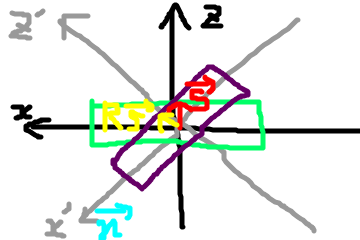
\includegraphics[width=0.8\columnwidth]{figs/section1/example}
  \caption{黒い座標を$W$の座標系,BODYリンクを想定した直方体がworld座標系の原点に最初あって(緑色の直方体),今はピッチ軸周りに45度回転して(灰色座標および紫色の直方体)いる状態.ここからさらに水色の軸$\boldsymbol{n}$周りに$\Delta \eta$回転しようとしている.はてなブログから持ってきたのであれだけど,黄色のベクトルが$\boldsymbol{p}^{A}$}
  \label{fig:example}
\end{figure}
このとき,
\begin{gather}
  {}^{W}_{A(t)}\boldsymbol{R} = \begin{pmatrix}
    \frac{1}{\sqrt{2}} & 0 & \frac{1}{\sqrt{2}}\\
    0 & 1 & 0\\
    -\frac{1}{\sqrt{2}} & 0 & \frac{1}{\sqrt{2}}
  \end{pmatrix}\\
  {}^{A(t)}_{A(t+\Delta t)}\boldsymbol{R} = \begin{pmatrix}
    1 & 0 & 0\\
    0 & \cos \Delta \eta & - \sin \Delta \eta\\
    0 & \sin \Delta \eta &   \cos \Delta \eta
  \end{pmatrix}\\
  \boldsymbol{p}^{A} = \begin{pmatrix}
    0\\
    0\\
    1
  \end{pmatrix}
\end{gather}
となる.
回転行列は\autoref{listing:matirx_from_euler}で求められる.

\lstinputlisting[language=Python, caption=matrix\_from\_euler.py, label=listing:matirx_from_euler, numbers=left, showstringspaces=false,
  keywordstyle={\bfseries \color[cmyk]{1,0,0.1,0}},
  stringstyle={\ttfamily \color[cmyk]{0.5,0,1,0}},
  basicstyle=\ttfamily\small]{codes/matrix_from_euler.py}

\autoref{eq:bibun}の左辺は
\begin{gather}
  \begin{align}
    \boldsymbol{p}^{W}_{t+ \Delta t} &= {}^{W}_{A(t+ \Delta t)}\boldsymbol{R}\boldsymbol{p}^{A}\\
    &= {}^{W}_{A(t)}\boldsymbol{R}{}^{A(t)}_{A(t+ \Delta t)}\boldsymbol{R}\boldsymbol{p}^{A}\\
    &= \begin{pmatrix}
      \frac{\cos \Delta \eta}{\sqrt{2}}\\
      - \sin \Delta \eta\\
      \frac{\cos \Delta \eta}{\sqrt{2}}
    \end{pmatrix}\\
    &\simeq \begin{pmatrix}
      \frac{1}{\sqrt{2}}\\
      - \Delta \eta\\
      \frac{1}{\sqrt{2}}
    \end{pmatrix}
  \end{align}\\
  \boldsymbol{p}^{W}_{t} = \begin{pmatrix}
    \frac{1}{\sqrt{2}}\\
    0\\
    \frac{1}{\sqrt{2}}
  \end{pmatrix}
\end{gather}
より,
\begin{align}
  \lim_{\Delta t \to 0} \frac{\boldsymbol{p}^{W}_{t+ \Delta t} - \boldsymbol{p}^{W}_{t}}{\Delta t} &= \begin{pmatrix}
    0\\
    -\frac{\Delta \eta}{\Delta t}\\
    0
  \end{pmatrix}
\end{align}\\
\autoref{eq:bibun}と\autoref{eq:result}から,$\boldsymbol{\omega}^{W}$は
\begin{equation}
  \boldsymbol{\omega}^{W} \times \begin{pmatrix}
    \frac{1}{\sqrt{2}}\\
    0\\
    \frac{1}{\sqrt{2}}
  \end{pmatrix} = \begin{pmatrix}
    0\\
    -\frac{\Delta \eta}{\Delta t}\\
    0
  \end{pmatrix}\label{eq:target}
\end{equation}
を満たすはず.
\begin{equation}
  \boldsymbol{\omega}^{A} = \begin{pmatrix}
    \frac{\Delta \eta}{\Delta t}\\
    0\\
    0
  \end{pmatrix}
\end{equation}
なので,
\begin{equation}
  \boldsymbol{\omega}^{W} = {}^{W}_{A(t)}\boldsymbol{R} \boldsymbol{\omega}^{A} = \begin{pmatrix}
    \frac{1}{\sqrt{2}} \frac{\Delta \eta}{\Delta t}\\
    0\\
    -\frac{1}{\sqrt{2}} \frac{\Delta \eta}{\Delta t}
  \end{pmatrix}
\end{equation}
であるが,これは\autoref{eq:target}を満たすので,合っている.

ジャイロセンサが感知するのは,$\boldsymbol{\omega}^{A}$の方.

\subsection{回転行列とRPYの関係}\label{subsec:rpy}
\subsubsection{証明}
\url{https://www.jstage.jst.go.jp/article/sicetr1965/40/11/40_11_1160/_pdf}が参考になるし,このテクニックはすごい気がする.

RPYは,オイラー角の一種で,Z$\to$Y$\to$Xの順番で軸周りに回転していくスタイル.
回転角度を順に,Yaw($\gamma$)$\to$Pitch($\beta$)$\to$Roll($\alpha$)と呼ぶ.
これを使って回転行列を表現すると
\begin{equation}
  \boldsymbol{R} = {\tiny \begin{pmatrix}
      \cos \beta \cos \gamma & \sin \alpha \sin \beta \cos \gamma - \cos \alpha \sin \gamma & \cos \alpha \sin \beta \cos \gamma + \sin \alpha \sin \gamma \\
      \cos \beta \sin \gamma & \sin \alpha \sin \beta \sin \gamma + \cos \alpha \cos \gamma & \cos \alpha \sin \beta \sin \gamma - \sin \alpha \cos \gamma \\
      -\sin \beta & \sin \alpha \cos \beta & \cos \alpha \cos \beta
  \end{pmatrix}}
\end{equation}
となる.

一方,$[\boldsymbol{\omega}]_{\times} = \dot{\boldsymbol{R}} \boldsymbol{R}^{T}$であり,
\begin{align}
  [\boldsymbol{\omega}]_{\times} &=
  \begin{pmatrix}
    0  & -\omega_{z} & \omega_{y}\\
    \omega_{z} & 0 & -\omega_{x}\\
    - \omega_{y}  & \omega_{x} & 0
  \end{pmatrix}\\
  &= \omega_{x} \boldsymbol{X}_1 + \omega_{y} \boldsymbol{X}_2 + \omega_{z} \boldsymbol{X}_3\\
  \boldsymbol{X}_1 &=
  \begin{pmatrix}
    0 & 0 & 0\\
    0 & 0 & -1\\
    0 & 1 & 0
  \end{pmatrix}\\
  \boldsymbol{X}_2 &=
  \begin{pmatrix}
    0 & 0 & 1\\
    0 & 0 & 0\\
    1 & 0 & 0
  \end{pmatrix}\\
  \boldsymbol{X}_3 &=
  \begin{pmatrix}
    0 & -1 & 0\\
    1 & 0 & 0\\
    0 & 0 & 0
  \end{pmatrix}
\end{align}
となって,ここで急に
\begin{gather}
  \boldsymbol{X}_1 \boldsymbol{X}_1 \boldsymbol{X}_1^{T} = \boldsymbol{X}_1\\
  \boldsymbol{X}_1 \boldsymbol{X}_2 \boldsymbol{X}_1^{T} = \boldsymbol{O}\\
  \boldsymbol{X}_1 \boldsymbol{X}_3 \boldsymbol{X}_1^{T} = \boldsymbol{O}
\end{gather}
という関係式を思いつくことができれば,
\begin{gather}
  \omega_{x} \boldsymbol{X}_1 = \boldsymbol{X}_1 [\boldsymbol{\omega}]_{\times} \boldsymbol{X}_1^{T}\\
  \omega_{y} \boldsymbol{X}_2 = \boldsymbol{X}_2 [\boldsymbol{\omega}]_{\times} \boldsymbol{X}_2^{T}\\
  \omega_{z} \boldsymbol{X}_3 = \boldsymbol{X}_3 [\boldsymbol{\omega}]_{\times} \boldsymbol{X}_3^{T}
\end{gather}
という境地に達する.
これを使うと,割と簡単に$[\boldsymbol{\omega}]_{\times} = \dot{\boldsymbol{R}} \boldsymbol{R}^{T}$をオイラー角の微分について整理することが可能になる.(この境地に達しないと,回転行列の微分をして,,,のようにゴリゴリ計算しないといけなくて,sympyを使ってもちょっと無理だった.)

どう簡単になるかというと,りあえず最初の式に注目すると,
\begin{align}
  & \omega_{x} \boldsymbol{X}_1 = \boldsymbol{X}_1 [\boldsymbol{\omega}]_{\times} \boldsymbol{X}_1^{T}\\
  \Leftrightarrow & \omega_{x} \boldsymbol{X}_1 = \boldsymbol{X}_1 \dot{\boldsymbol{R}} \boldsymbol{R}^{T} \boldsymbol{X}_1^{T}\\
  \Leftrightarrow & \omega_{x} \boldsymbol{X}_1 = \left(\boldsymbol{X}_1 \dot{\boldsymbol{R}}\right) \left(\boldsymbol{X}_1 \boldsymbol{R}\right)^{T}
\end{align}
が成り立つ.
\begin{equation}
  \boldsymbol{R} = \begin{pmatrix}
      a_{11} & a_{12} & a_{13}\\
      a_{21} & a_{22} & a_{23}\\
      a_{31} & a_{32} & a_{33}
  \end{pmatrix}
\end{equation}
と置くと,
\begin{align}
  & \omega_{x} \boldsymbol{X}_1 = \left(\boldsymbol{X}_1 \dot{\boldsymbol{R}}\right) \left(\boldsymbol{X}_1 \boldsymbol{R}\right)^{T}\\
  \Leftrightarrow & \omega_{x} \boldsymbol{X}_1 =
  \begin{pmatrix}
    0 & 0 & 0\\
    - \dot{a}_{31} & - \dot{a}_{32} & - \dot{a}_{33}\\
    \dot{a}_{21} & \dot{a}_{22} & \dot{a}_{23}
  \end{pmatrix}
  \begin{pmatrix}
    0 & - a_{31} & a_{21}\\
    0 & - a_{32} & a_{22}\\
    0 & - a_{33} & a_{23}
  \end{pmatrix}\\
  \Leftrightarrow & \omega_{x} \boldsymbol{X}_1 =
  {\tiny \begin{pmatrix}
      0 & 0 & 0\\
      0 & \dot{a}_{31} a_{31} + \dot{a}_{32} a_{32} + \dot{a}_{33} a_{33} & - \dot{a}_{31} a_{21} - \dot{a}_{32} a_{22} - \dot{a}_{33} a_{23}\\
      0 & - a_{31} \dot{a}_{21} - a_{32} \dot{a}_{22} - a_{33} \dot{a}_{23} & \dot{a}_{21} a_{21} + \dot{a}_{22} a_{22} + \dot{a}_{23} a_{23}
  \end{pmatrix}}
\end{align}
ここで,回転行列の性質$a_{31}^2 + a_{32}^2 + a_{33}^2=1$と$a_{31} a_{21} + a_{32} a_{22} + a_{33} a_{23} = 0$より,微分して,$\dot{a}_{31} a_{31} + \dot{a}_{32} a_{32} + \dot{a}_{33} a_{33} = 0$と$\dot{a}_{31} a_{21} + \dot{a}_{32} a_{22} + \dot{a}_{33} a_{23} = - a_{31} \dot{a}_{21} - a_{32} \dot{a}_{22} - a_{33} \dot{a}_{23}$なので,
\begin{align}
  & \omega_{x} \boldsymbol{X}_1 =
  {\tiny \begin{pmatrix}
      0 & 0 & 0\\
      0 & \dot{a}_{31} a_{31} + \dot{a}_{32} a_{32} + \dot{a}_{33} a_{33} & - \dot{a}_{31} a_{21} - \dot{a}_{32} a_{22} - \dot{a}_{33} a_{23}\\
      0 & - a_{31} \dot{a}_{21} - a_{32} \dot{a}_{22} - a_{33} \dot{a}_{23} & \dot{a}_{21} a_{21} + \dot{a}_{22} a_{22} + \dot{a}_{23} a_{23}
  \end{pmatrix}}\\
  \Leftrightarrow & \omega_{x} \boldsymbol{X}_1 =
  {\tiny
    \begin{pmatrix}
      0 & 0 & 0\\
      0 & 0 & - \dot{a}_{31} a_{21} - \dot{a}_{32} a_{22} - \dot{a}_{33} a_{23}\\
      0 & \dot{a}_{31} a_{21} + \dot{a}_{32} a_{22} + \dot{a}_{33} a_{23} & 0
  \end{pmatrix}}\\
  \Leftrightarrow &
  \omega_{x} \boldsymbol{X}_1 =
  (\dot{a}_{31} a_{21} + \dot{a}_{32} a_{22} + \dot{a}_{33} a_{23}) \boldsymbol{X}_1\\
  \Leftrightarrow & \omega_{x} = \dot{a}_{31} a_{21} + \dot{a}_{32} a_{22} + \dot{a}_{33} a_{23}
\end{align}
これはすごい.
他の項にも適用して,
\begin{align}
  \omega_{x} &= \dot{a}_{31} a_{21} + \dot{a}_{32} a_{22} + \dot{a}_{33} a_{23}\\
  \omega_{y} &= \dot{a}_{11} a_{31} + \dot{a}_{12} a_{32} + \dot{a}_{13} a_{33}\\
  \omega_{z} &= \dot{a}_{21} a_{11} + \dot{a}_{22} a_{12} + \dot{a}_{23} a_{13}
\end{align}
となる.
これを,今回注目しているZ-Y-Xオイラー角に当てはめて整理すると(これもなかなか大変...)
\begin{align}
  & \begin{pmatrix}
      \omega_{x}\\
      \omega_{y}\\
      \omega_{z}
    \end{pmatrix} =
  \begin{pmatrix}
    \cos \beta \cos \gamma & - \sin \gamma & 0 \\
    \cos \beta \sin \gamma &   \cos \gamma & 0 \\
    - \sin \beta &             0 & 1
  \end{pmatrix}
  \begin{pmatrix}
    \dot{\alpha}\\
    \dot{\beta}\\
    \dot{\gamma}
  \end{pmatrix}\\
  \Leftrightarrow & \boldsymbol{\omega}^{W} =
  \begin{pmatrix}
    \cos \beta \cos \gamma & - \sin \gamma & 0 \\
    \cos \beta \sin \gamma &   \cos \gamma & 0 \\
    - \sin \beta &             0 & 1
  \end{pmatrix}
  \begin{pmatrix}
    \dot{\alpha}\\
    \dot{\beta}\\
    \dot{\gamma}
  \end{pmatrix}
\end{align}
$\boldsymbol{\omega}^{A}$を求めるために,両辺左から${}^{W}_{A}\boldsymbol{R}^{T}$をかけて整理すると
\begin{equation}
  \boldsymbol{\omega}^{A} =
  \begin{pmatrix}
    1 & 0 & - \sin \beta \\
    0 & \cos \alpha & \sin \alpha \cos \beta \\
    0 & - \sin \alpha & \cos \alpha \cos \beta
  \end{pmatrix}
  \begin{pmatrix}
    \dot{\alpha}\\
    \dot{\beta}\\
    \dot{\gamma}
  \end{pmatrix}
\end{equation}

ちなみに,\autoref{listing:rotation_matirx}で検証可能.

\lstinputlisting[language=Python, caption=rotation\_matrix.py, label=listing:rotation_matirx, numbers=left, showstringspaces=false,
  keywordstyle={\bfseries \color[cmyk]{1,0,0.1,0}},
  stringstyle={\ttfamily \color[cmyk]{0.5,0,1,0}},
  basicstyle=\ttfamily\small]{codes/rotation_matrix.py}

この逆は
\begin{equation}
  \begin{pmatrix}
    \dot{\alpha}\\
    \dot{\beta}\\
    \dot{\gamma}
  \end{pmatrix} =
  \begin{pmatrix}
    1 & \frac{\sin \alpha \sin \beta}{\cos \beta} & \frac{\cos \alpha \sin \beta}{\cos \beta} \\
    0 & \cos \alpha & - \sin \alpha \\
    0 & \frac{\sin \alpha}{\cos \beta} & \frac{\cos \alpha}{\cos \beta}
  \end{pmatrix}
  \boldsymbol{\omega}^{A}
\end{equation}
となる\footnote{\url{http://www.wolframalpha.com/input/?i=Inverse\%5B\%7B\%7B1\%2C0\%2C-sin\%28b\%29\%7D\%2C\%7B0\%2Ccos\%28a\%29\%2C+sin\%28a\%29*cos\%28b\%29\%7D\%2C\%7B0\%2C-sin\%28a\%29\%2C+cos\%28a\%29+*+cos\%28b\%29\%7D\%7D\%5D}}.

\subsubsection{具体例で実験}
\autoref{subsubsec:test1}と同じシチュエーションを考える.
角速度を求めようとすると
\begin{equation}
  \begin{pmatrix}
    \alpha \\
    \beta \\
    \gamma
  \end{pmatrix} =
  \begin{pmatrix}
    0 \\
    \frac{\pi}{4} \\
    0
  \end{pmatrix}
\end{equation}
なので
\begin{equation}
  \boldsymbol{\omega}^{W} =
  \begin{pmatrix}
    \frac{\sqrt{2}}{2} & 0 & 0 \\
    0 & 1 & 0 \\
    - \frac{\sqrt{2}}{2} & 0 & 1
  \end{pmatrix}
  \begin{pmatrix}
    \dot{\alpha} \\
    0 \\
    0
  \end{pmatrix} =
  \begin{pmatrix}
    \frac{\sqrt{2}}{2} \dot{\alpha} \\
    0 \\
    -\frac{\sqrt{2}}{2} \dot{\alpha}
  \end{pmatrix}
\end{equation}
\begin{equation}
  \boldsymbol{\omega}^{A} =
  \begin{pmatrix}
    1 & 0 & - \frac{\sqrt{2}}{2} \\
    0 & 1 & 0 \\
    0 & 0 & \frac{\sqrt{2}}{2}
  \end{pmatrix}
  \begin{pmatrix}
    \dot{\alpha} \\
    0 \\
    0
  \end{pmatrix} =
  \begin{pmatrix}
    \dot{\alpha} \\
    0 \\
    0
  \end{pmatrix}
\end{equation}
となり,確かに直感と合う.

また,別のシチュエーションとして,
ヨー方向に90度回転させた後に,world座標のピッチ方向に回転させた場合は,
\begin{equation}
  \begin{pmatrix}
    \alpha \\
    \beta \\
    \gamma
  \end{pmatrix} =
  \begin{pmatrix}
    0 \\
    0 \\
    \frac{\pi}{2}
  \end{pmatrix}
\end{equation}
のとき,
\begin{equation}
  \boldsymbol{\omega}^{W} =
  \begin{pmatrix}
    0 & -1 & 0\\
    1 & 0 & 0\\
    0 & 0 & 1
  \end{pmatrix}
  \begin{pmatrix}
    \dot{\alpha} \\
    0 \\
    0
  \end{pmatrix} =
  \begin{pmatrix}
    0 \\
    \dot{\alpha} \\
    0
  \end{pmatrix}
\end{equation}
\begin{equation}
  \boldsymbol{\omega}^{A} =
  \begin{pmatrix}
    1 & 0 & 0\\
    0 & 0 & 1\\
    0 & -1 & 0
  \end{pmatrix}
  \begin{pmatrix}
    \dot{\alpha} \\
    0 \\
    0
  \end{pmatrix} =
  \begin{pmatrix}
    \dot{\alpha} \\
    0 \\
    0
  \end{pmatrix}
\end{equation}
となり,確かに直感と合う.

\subsection{回転行列とQuaternionの関係}\label{subsec:quat}
\url{http://www.mss.co.jp/technology/report/pdf/18-07.pdf}が参考になる.

\subsubsection{クォータニオンの定義}
スカラー部を$q_0$,ベクトル部を$\boldsymbol{q} = (q_1, q_2, q_3)$として,
$\tilde{\boldsymbol{q}} = (q_0, \boldsymbol{q})$とする.

回転クォータニオンは
\begin{equation}
  \tilde{\boldsymbol{q}} = \cos \frac{\theta}{2} + \left(u_x \boldsymbol{i} + u_y \boldsymbol{j} + u_z \boldsymbol{k}\right) \sin \frac{\theta}{2}
\end{equation}
で,とある座標系$B$で表現された位置ベクトル$\boldsymbol{a}$を座標系は動かさずに位置ベクトルだけ回転させるときは$\boldsymbol{a}^{B}_{t+1} = \tilde{\boldsymbol{q}} \boldsymbol{a}^{B}_{t} \tilde{\boldsymbol{q}^{\ast}}$で,座標系を動かして位置ベクトルの先っぽにある点は動かさないときは$\boldsymbol{a}^{B_{t+1}} = \tilde{\boldsymbol{q}} \boldsymbol{a}^{B_{t}} \tilde{\boldsymbol{q}^{\ast}}$となる.

ベクトルと掛け算するときは$\boldsymbol{a}=(a_x, a_y, a_z)$を$a_x \boldsymbol{i} + a_y \boldsymbol{j} + a_z \boldsymbol{k}$と見なして計算するというのがミソ\footnote{\url{http://mathtrain.jp/quaternion}}.例えば$(3,0,0)$を$x=z,y=0$の軸周りに60度回すとすると,回転クォータニオンは$\tilde{\boldsymbol{q}} = \frac{\sqrt{3}}{2} + \left(\frac{1}{\sqrt{2}} \boldsymbol{i} + \frac{1}{\sqrt{2}} \boldsymbol{k}\right) \frac{1}{2} = \frac{\sqrt{3}}{2} + \frac{1}{2\sqrt{2}} \boldsymbol{i} + \frac{1}{2\sqrt{2}} \boldsymbol{k}$なので,
{\tiny
  \begin{align}
    \tilde{\boldsymbol{q}} \boldsymbol{a}^{B}_{t} \tilde{\boldsymbol{q}^{\ast}} &= \left(\frac{\sqrt{3}}{2} + \frac{1}{2\sqrt{2}} \boldsymbol{i} + \frac{1}{2\sqrt{2}} \boldsymbol{k}\right) \cdot 3 \boldsymbol{i} \cdot \left(\frac{\sqrt{3}}{2} - \frac{1}{2\sqrt{2}} \boldsymbol{i} - \frac{1}{2\sqrt{2}} \boldsymbol{k}\right)\\
    &= \left(\frac{3\sqrt{3}}{2}\boldsymbol{i} - \frac{3}{2\sqrt{2}} + \frac{3}{2\sqrt{2}} \boldsymbol{j}\right) \cdot \left(\frac{\sqrt{3}}{2} - \frac{1}{2\sqrt{2}} \boldsymbol{i} - \frac{1}{2\sqrt{2}} \boldsymbol{k}\right)\\
    &= \left(\frac{9}{4}\boldsymbol{i} + \frac{3\sqrt{3}}{4\sqrt{2}} + \frac{3\sqrt{3}}{4\sqrt{2}} \boldsymbol{j}\right) +
    \left(-\frac{3\sqrt{3}}{4\sqrt{2}} + \frac{3}{8}\boldsymbol{i} + \frac{3}{8}\boldsymbol{k}\right) +
    \left(\frac{3\sqrt{3}}{4\sqrt{2}}\boldsymbol{j} + \frac{3}{8}\boldsymbol{k} - \frac{3}{8}\boldsymbol{i}\right)\\
    &= \frac{9}{4}\boldsymbol{i} + \frac{3\sqrt{3}}{2\sqrt{2}}\boldsymbol{j} + \frac{3}{4}\boldsymbol{k}
  \end{align}
}
となって,回転後は$(\frac{9}{4}, \frac{3\sqrt{3}}{2\sqrt{2}}, \frac{3}{4})$となる.

一般的にもできて,クォータニオンのベクトル部の掛け算は$\boldsymbol{u} \boldsymbol{j} = - \boldsymbol{u} \cdot \boldsymbol{j} + \boldsymbol{u} \times \boldsymbol{j}$なので
{\tiny
  \begin{align}
    \boldsymbol{a}^{B}_{t+1} &= \tilde{\boldsymbol{q}} \boldsymbol{a}^{B}_{t} \tilde{\boldsymbol{q}^{\ast}}\\
    &= \left(\cos \frac{\theta}{2} + \boldsymbol{u} \sin \frac{\theta}{2}\right) \boldsymbol{a} \left(\cos \frac{\theta}{2} - \boldsymbol{u} \sin \frac{\theta}{2}\right)\\
    &= \left(\cos \frac{\theta}{2} \boldsymbol{a} - \boldsymbol{u} \cdot \boldsymbol{a} \sin \frac{\theta}{2} + \boldsymbol{u} \times \boldsymbol{a} \sin \frac{\theta}{2}\right) \left(\cos \frac{\theta}{2} - \boldsymbol{u} \sin \frac{\theta}{2}\right)\\
    &= \left\{- \boldsymbol{u} \cdot \boldsymbol{a} \sin \frac{\theta}{2} + \left( \cos \frac{\theta}{2} \boldsymbol{a}  + \boldsymbol{u} \times \boldsymbol{a} \sin \frac{\theta}{2}\right)\right\} \left(\cos \frac{\theta}{2} - \boldsymbol{u} \sin \frac{\theta}{2}\right)\\
    &= - \boldsymbol{u} \cdot \boldsymbol{a} \frac{\sin \theta}{2}
    + \boldsymbol{u} \cdot \boldsymbol{a} \sin^2 \frac{\theta}{2} \boldsymbol{u}
    + \left( \cos \frac{\theta}{2} \boldsymbol{a}  + \boldsymbol{u} \times \boldsymbol{a} \sin \frac{\theta}{2}\right) \left(\cos \frac{\theta}{2} - \boldsymbol{u} \sin \frac{\theta}{2}\right)\\
    &= \left(\boldsymbol{u} \cdot \boldsymbol{a}\right)\boldsymbol{u} + \left\{\boldsymbol{a} - \left(\boldsymbol{u} \cdot \boldsymbol{a}\right)\boldsymbol{u}\right\} \cos \theta + \boldsymbol{u} \times \boldsymbol{a} \sin \theta
  \end{align}
}
となって,綺麗にベクトル部だけ残る.

\subsubsection{クォータニオンの定義}
あるベクトル$\boldsymbol{a}_{t}$があって,回っていて,
$t=t$のときのクォータニオンを$\tilde{\boldsymbol{q}}_{t}$,
$t=t+\Delta t$のときのクォータニオンを$\tilde{\boldsymbol{q}}_{t+\Delta t}$とすると,
\begin{align}
  \boldsymbol{a}_{t+\Delta t} &= \tilde{\boldsymbol{q}}_{t+\Delta t} \boldsymbol{a}_{0} \tilde{\boldsymbol{q}}_{t+\Delta t}^{\ast}\\
  &= \tilde{\boldsymbol{\Delta q}} \boldsymbol{a}_{t} \tilde{\boldsymbol{\Delta q}}^{\ast}\\
  &= \tilde{\boldsymbol{\Delta q}} \tilde{\boldsymbol{q}}_{t} \boldsymbol{a}_{0} \tilde{\boldsymbol{q}}_{t}^{\ast} \tilde{\boldsymbol{\Delta q}}^{\ast}
\end{align}
となるので,
\begin{equation}
  \tilde{\boldsymbol{q}}_{t+\Delta t}= \tilde{\boldsymbol{\Delta q}} \tilde{\boldsymbol{q}}_{t}
\end{equation}
となる.
ここで,$\tilde{\boldsymbol{\Delta q}}$は$\boldsymbol{s}^{W}$周りに微少量$\Delta \theta$だけ回転させたものと考えられて,
\begin{equation}
  \tilde{\boldsymbol{\Delta q}} = \cos \frac{\Delta \theta}{2} + \frac{\boldsymbol{s}^{W}}{\lVert \boldsymbol{s}^{W} \rVert} \sin \frac{\Delta \theta}{2} \simeq 1 + \frac{1}{2} \frac{\boldsymbol{s}^{W}}{\lVert \boldsymbol{s}^{W} \rVert} \Delta \theta
\end{equation}
となるので,
\begin{align}
  \dot{\tilde{\boldsymbol{q}}}_{t} &= \frac{\tilde{\boldsymbol{q}}_{t+\Delta t} - \tilde{\boldsymbol{q}}_{t}}{\Delta t}\\
  &= \frac{\tilde{\boldsymbol{\Delta q}} \tilde{\boldsymbol{q}}_{t} - \tilde{\boldsymbol{q}}_{t}}{\Delta t}\\
  &= \frac{\left(1 + \frac{1}{2} \frac{\boldsymbol{s}^{W}}{\lVert \boldsymbol{s}^{W} \rVert} \Delta \theta\right) \tilde{\boldsymbol{q}}_{t} - \tilde{\boldsymbol{q}}_{t}}{\Delta t}\\
  &= \frac{1}{2} \frac{\boldsymbol{s}^{W}}{\lVert \boldsymbol{s}^{W} \rVert} \frac{\Delta \theta}{\Delta t} \tilde{\boldsymbol{q}}_{t}\\
  &= \frac{1}{2} \boldsymbol{\omega}^{W} \tilde{\boldsymbol{q}}_{t}
\end{align}
と分かる.
行列形式で表現すると
{\tiny
  \begin{align}
    \dot{\tilde{\boldsymbol{q}}}_{t} &= \frac{1}{2} \boldsymbol{\omega}^{W} \tilde{\boldsymbol{q}}_{t}\\
    &= \frac{1}{2}
    \begin{pmatrix}
      \omega_X\\
      \omega_Y\\
      \omega_Z
    \end{pmatrix}
    \left\{q_0 +
    \begin{pmatrix}
      q_1\\
      q_2\\
      q_3
    \end{pmatrix}\right\}\\
    &= \frac{1}{2}
    \left\{
    q_0
    \begin{pmatrix}
      \omega_X\\
      \omega_Y\\
      \omega_Z
    \end{pmatrix}
    - \left( \omega_X q_1 + \omega_Y q_2 + \omega_Z q_3 \right) +
    \begin{pmatrix}
      \omega_Y q_3 - \omega_Z q_2\\
      \omega_Z q_1 - \omega_X q_3\\
      \omega_X q_2 - \omega_Y q_1
    \end{pmatrix}\right\}\\
    &= \frac{1}{2}
    \begin{pmatrix}
      0 & - \omega_X & - \omega_Y & - \omega_Z\\
      \omega_X & 0 & -\omega_Z & \omega_Y\\
      \omega_Y & \omega_Z & 0 & -\omega_X\\
      \omega_Z & - \omega_Y & \omega_X & 0
    \end{pmatrix}
    \begin{pmatrix}
      q_0\\
      q_1\\
      q_2\\
      q_3
    \end{pmatrix}
  \end{align}
}
となる.

しかし,$\boldsymbol{\omega}^{W}$はworld座標系で表された角速度で,
IMUが観測するのはlocal座標で表された角速度なので,
ベクトルの回転ではなくて座標系の回転であるためにクォータニオンの順番が変わることに注意しつつ
\begin{align}
  & \boldsymbol{\omega}^{A} = \tilde{\boldsymbol{q}}^{\ast}_{t} \boldsymbol{\omega}^{W} \tilde{\boldsymbol{q}}_{t}\\
  \Leftrightarrow& \boldsymbol{\omega}^{W} = \tilde{\boldsymbol{q}}_{t} \boldsymbol{\omega}^{A} \tilde{\boldsymbol{q}}^{\ast}_{t}
\end{align}
と変換しなくてはいけない.

そうすると
\begin{align}
  \dot{\tilde{\boldsymbol{q}}}_{t} &= \frac{1}{2} \boldsymbol{\omega}^{W} \tilde{\boldsymbol{q}}_{t}\\
  &= \frac{1}{2} \tilde{\boldsymbol{q}}_{t} \boldsymbol{\omega}^{A} \tilde{\boldsymbol{q}}^{\ast}_{t} \tilde{\boldsymbol{q}}_{t}\\
    &= \frac{1}{2} \tilde{\boldsymbol{q}}_{t} \boldsymbol{\omega}^{A}
\end{align}

これを行列形式で書くと
\begin{equation}
  \dot{\tilde{\boldsymbol{q}}}_{t} =
  \frac{1}{2}
  \begin{pmatrix}
    0        & -\omega_x & -\omega_y & -\omega_z\\
    \omega_x &         0 &  \omega_z & -\omega_y\\
    \omega_y & -\omega_z &         0 &  \omega_x\\
    \omega_z &  \omega_y &  \omega_x &         0
  \end{pmatrix}
  \begin{pmatrix}
    q_0\\
    q_1\\
    q_2\\
    q_3
  \end{pmatrix}
\end{equation}
のように中身がちょっと変わるので,注意.

\subsection{加速度と回転の関係}\label{subsec:acc}
